% !TeX root = ../main.tex
% 原始章节：11-advenced-cpu.Rmd

\chapter{处理器性能优化}\label{chap:11-advanced-cpu}

对于处理器运行特定测试程序时的性能，通常以执行时间对其进行评价。
对于相同的体系结构，运行特定程序可以视为执行了相同的指令序列。因此对特定测试程序和特定体系结构，程序的执行时间与只与处理器每单位时间内可以执行的指令数量相关。

因此要改提升通用处理器性能，实际就是提高处理器执行指令的吞吐量。
处理器每单位时间内可以执行的指令数量，实际就等于处理器的运行频率乘以平均每周期执行的指令数。
提高处理器性能即提高处理器的运行频率、提高处理器每周期执行的指令数（IPC）。

\section{处理器运行频率优化}\label{sec:11-advanced-cpu-001}

\subsection{存储部件优化}\label{sec:11-advanced-cpu-002}

处理器内部，存在大量的存储部件。如指令缓存、数据缓存、跳转目标地址缓冲器等等。
这些存储部件，随着处理器规模扩大，往往也有较大的容量和低延迟需求。
这些存储部件常使用 SRAM 实现。 SRAM 存储单元由六个晶体管组成，其中内部四个晶体管组成两个反相器。
这两个反相器耦合，形成一个环路。在无其它输入的情况下保持稳态，整体对外表现为弱驱动。
SRAM 中的另外两个晶体管，用于控制从 SRAM 中读出数据，或通过外部强驱动破坏内部弱驱动稳态，写入新的数据。

SRAM 器件的输出，来自内部六管晶体管组成的两个耦合反相器。且为了保证外部强驱动可以写入新数据，两个耦合反相器输出高电平的驱动能力往往较弱。
SRAM 部件的特殊特性，导致其速度一定慢于锁存器结构的数据存储单元。

处理器内部，大量的大容量 SRAM ，往往会成为处理器频率的一个瓶颈。为了解决这种瓶颈，处理器设计者需要从两个角度对设计进行优化。
首先，可以优化存储部件本身。如一些商业处理器设计者，会对 SRAM 进行全定制设计，以牺牲面积或者静态功耗为代价，加强 SRAM 驱动性能等，根据处理器实际需求寻找一个均衡的设计点。
不具备相似定制设计条件下，可以在设计中规避时序较差的存储部件，如延长读取写入占用的周期数等等，以避免存储部件中占用过大的时序，造成设计时序紧张。

现代处理器，往往也具有大量的大容量多口寄存器堆设计。这些寄存器堆往往占用面积大、功耗大、时序糟糕。
对寄存器堆进行定制设计，也是处理器运行频率优化的重要环节之一。
和 SRAM 一样，商业处理器设计者对于寄存器堆，往往会进行定制设计。根据需要的容量和端口数量以及尺寸约束时序约束，绘制专门的存储单元，控制单元，生成版图。
若不具备定制条件的条件，仅能进行逻辑综合，也应在 RTL 级别尝试对寄存器堆进行一些优化。
寄存器堆的面积，往往与写端口数量的平方成正比。而过大的面积，会带来较困难的布线进一步影响寄存器堆运行频率。
因此，对于设计者来说，尽量使用容量较小、端口较少的寄存器堆也是频率优化的重要环节之一。

有时，处理器出于性能考虑，不得不需要使用多口寄存器堆，这时可以尝试复制的策略构建多口寄存器堆以优化时序和面积情况。

对于多读端口，由于读的操作是幂等的，只需要简单的复制多组相同写端口数量的寄存器堆即可，读取端口自然得到了倍增。
但对于非幂等的写端口，多端口设计则较麻烦。一种常用的方案是 LVT（Live Value Table），使用小容量多写口寄存器堆与多个单写口寄存器堆构建多写口寄存器堆。
这种方案中，有多少个写端口，就复制几组寄存器堆。同时准备一个真多写口的小容量寄存器堆（LVT）记录最新的值位于哪个寄存器堆中。

在读写端口之外，对存储单元的优化也较为重要。每个存储单元记录一位数据，对于寄存器堆而言，存储单元的复杂度和面积占用，决定了整体的面积和时序情况。
即使无法进行专门的定制设计，也可以进行半定制操作，直接使用标准单元结构描述寄存器堆，及实际存储单元。
如，可以直接使用锁存器，避免使用寄存器组成寄存器堆。锁存器与寄存器均可存储数据，但可节约一半的晶体管。
半定制设计，可以直接采用厂家提供的标准单元库完成整个寄存器堆的搭建，以实现频率和面积的优化。当然完成相应设计后，需要进行更为复杂的时序和功能正确性验证。

\subsection{平衡各级流水线的延迟}\label{sec:11-advanced-cpu-003}

体系结构设计中，存在明显的``木桶效应''。处理器性能的瓶颈，往往受制于最短板的一部分。
对于处理器频率的优化也是一样的。处理器频率，只受制于流水线中，时序最紧张的一级。
因此，对于一个确定的微架构，整体逻辑复杂度是确定的。根据简单的不等式关系可以知道，只有当每级流水线延迟均近似相等时，处理器才有最优的运行频率。

这一部分，需要频繁的结合逻辑综合工具，及后端布局布线的时序反馈，对设计进行反思改进。当然，一些过往设计的经验也值得参考。
现有的商业处理器，一般有较为均匀的流水线切分策略，也可以对这些成熟的微体系结构进行参考。
但整体而言，依然是一个需要在实践中发现理解的过程。多编码，多综合，多查看报告是唯一可行路径。

需要注意的是，最终目标并不是需要处理器主频尽可能高，而是要各个寄存器之间切分的组合逻辑时序尽可能接近。
如果一个设计中，某一级流水线成为时序瓶颈，且难以进一步拆分或者优化，那一种可能的正确选择是尝试合并其它流水级，创建尽可能平均的时序延迟分布。
较短的流水线，往往意味着更短的指令执行延迟，更快的分支响应速度。也对性能有很大正面的帮助。

\subsection{弹性流水线}\label{sec:11-advanced-cpu-004}

在很多的流水线设计中，较长的 ready 前馈信号组合逻辑链是限制频率的一大因素。
流水线中，每一级拉高前级流水线 ready 信号的条件，是本级流水线空或者下级流水线 ready 拉高且未阻塞。

这就带来一个问题，每一级流水线的 ready 信号均依赖下一级流水线的 ready 信号。
可若直接去除这个依赖，仅当本级流水线空的时候才拉高 ready 信号，那么流水线中又会出现一半的空泡，严重限制流水线的性能。

因此在实践中，我们往往会构建弹性流水线。所谓弹性流水线，即使用一些先入先出队列（FIFO），替换原有的流水线寄存器。
对于 FIFO 而言，反馈给前级的流水线就绪信号，可以仅与当前 FIFO 容量相关。同时，只要 FIFO 容量大于等于 2，则处理器依然可以保持相同的满速率无空泡运行。
使用 FIFO 替代流水线寄存器，打断 ready 前馈级连构建弹性流水线，也是处理器频率优化的一大必备措施。

\subsection{逻辑复制}\label{sec:11-advanced-cpu-005}

处理器设计中，会出现部分电路具有较大的 FANOUT 的现象。较大的 FANOUT 带来较高的线负载，受限于逻辑元件的驱动能力也会降低处理器频率。
一种做法是，为 FANOUT 严重的关键电路进行逻辑复制，降低 FANOUT 提高处理器频率。

除了 FANOUT 的情况，还有一些时候，电路会由于布局问题带来严重的时序瓶颈。
如 TLB 设计，如指令和数据访存共用同一套 TLB 组件。指令和数据访存由于设计自身原因，在布局上距离较远。
如果两套距离较远的逻辑同时调用 TLB 组件，那么 TLB 组件的布局也将成为一大问题。
这里一般也会采用逻辑复制，将 TLB 复制一份，避免较远的布局复杂度。

逻辑复制，往往会带来较大的面积和功率开销。因此在使用相应的思路对电路优化前，一定要再三进行权衡。只有在非做不可的情况下，再进行相应的工作。

\section{超标量技术}\label{sec:11-advanced-cpu-006}

前文提到，处理器的性能由每周期可执行的指令数（IPC） * 运行频率决定。因此，提高处理器每周期可以执行的指令数也是提高处理器性能的一大方法。
处理器设计者们，因此引入了超标量执行技术，允许流水线在一个周期内执行多于一条指令，以提高处理器的性能。

\subsection{超标量设计引入的冲突及解决}\label{sec:11-advanced-cpu-007}

对比顺序标量核心，超标量核心其实只是多具备了每周期执行更多指令的能力。对比标量核心，超标量顺序核心可以认为只是增加了一条指令执行流水而已。

当然，每周期执行两条指令的流水线承载能力，会导致流水线中引入更多的数据冲突、控制冲突、结构冲突。我们首先对这些冲突，及其解除进行简介

\subsubsection{数据冲突}\label{sec:11-advanced-cpu-008}

新引入的数据冲突主要是在每周期同时送入管线执行的两条指令之间发生的。

同时执行的两条指令可能存在 RAW 的数据真依赖，即第二条指令依赖第一条指令执行结果，则第二条指令一定需要等待第一条指令执行结束后才能开始执行。

两条指令也可能存在 WAW 或者 WAR 的数据伪依赖。对于 WAR 的情况，需要注意前序的读不能读到后续指令写的结果。对于 WAW 的冲突，需要注意写入寄存器的值为最新值。

对于 WAW 及 WAR 冲突，在顺序执行的超标量流水线中稍加注意就不会导致问题，但对于 RAW 的真依赖，则需要特别注意和处理。

一种常见的解决方案是阻止两条存在 RAW 真依赖的指令同时发射执行。一些特殊的处理器，对于一些特殊的相关指令，也允许两条指令同时执行，在执行过程中解决真依赖问题。

\subsubsection{控制冲突}\label{sec:11-advanced-cpu-009}

新引入的指令，也为处理器控制流的处理带来了困难。比如两条同时发射的指令均为跳转指令、两条同时发射的指令均发生了异常跳转等等，这里有比较多可能的特殊情况。

一种可能的设计方案是实现比较复杂的检查机制，允许两条指令同时发出控制流转移请求，综合两条指令的控制流转移请求情况，使用一套比较复杂的组合逻辑确定两条指令如果按顺序执行的结果如何，并采用顺序执行的结果进行执行。

另一种可能的设计方案是限制控制冲突发生。即处理器核心虽支持每周期发射执行两条指令，但其中仅有一条指令允许发生分支或异常，另外一条流水线只允许执行一定不发生异常中断或者跳转的指令。

如此一来，在控制流转移方面的设计，超标量处理器就与标量处理器没有任何区别，不用再考虑复杂的特殊情况去做单独的处理了。

\subsubsection{结构冲突}\label{sec:11-advanced-cpu-010}

处理器实际执行的指令分布往往是不均匀的，整数的简单计算（加减与或）会比乘除有更高的出现频率，而乘除法又比较占用硬件的资源。
因此，在硬件设计中，对于较少执行的指令，往往只会提供少于流水线最大宽度的单元数量和吞吐能力。若处理器要在同一个周期执行的两条乘除指令，就存在结构冲突。

对于结构冲突的解决也比较简单，在静态调度的超标量处理器中，处理器核不允许两条存在结构冲突的指令同时发射，以此规避了所有可能的结构冲突存在。

对于超标量处理器，一般我们定义其宽度为流水线中最窄的一级。因此，保证整个流水线中的通路宽度，保证流水线各处均不窄于设计宽度是设计超标量处理器的关键一步。

\subsection{双取指设计}\label{sec:11-advanced-cpu-011}

在标量处理器中，取指单元只需要每周期产生一个 PC ，并根据 PC 完成取指，拿到一条指令即可。对于超标量处理器，每周期需要产生至少两个预计将连续执行的指令，并获取其值才可以。

在前面的设计中，我们已经介绍了 Cache 的实现，处理器核的取指一般也直接来自 Cache。我们先不介绍如何获取多个预期将连续执行的指令地址，这是分支预测器的工作，先假设每次传入取指模块的两个 PC，是紧连的两个指令字。

若两个指令字地址处于同一 Cache 行，则其命中情况一定相同，请求一命中，则请求二一定命中。这种情况下，我们可以增加对于 data ram 的读端口数量，保证两个不同 PC 上的请求都可以读到其请求。

若两个指令字地址处于不同的 Cache 行，则其命中情况不一定一致，若涉及跨页的情况，其可能也需要经历不同的地址翻译阶段。

对于这种不同行的地址，我们自然也可以通过复制一份 Cache 完成对其并发访问的支持。但 Cache 及地址翻译模块往往占用较多的面积，可能并不适合仅为了处理一些边界情况就做这种规模的复制。

在超标量处理器涉及中，我们可以简单直接的对这些边界情况加以限制。
有一种节约硬件资源，极端的设计。即要求每个请求对（两个 PC 请求）一定是双字对齐的。此时，取指模块直接将其作为一个双字访问来处理。

如此一来，指令缓存的数据部分不用额外增加访问端口，取指单元每周期仅需要处理一个对齐的取指请求，只不过这个请求是双字宽度的。

只需要在分支预测，或者 PC 生成部分，限制每次生成的 PC 对一定满足对齐要求即可。

\subsection{多口 FIFO 设计}\label{sec:11-advanced-cpu-012}

对于取指出来的两条指令，将会经历解码后送入后端执行。取指到解码发射执行之间，一般存在一个解码队列。由于一些指令之间存在数据冲突或者控制/结构冲突，不能同时发射
（仅能发射其中一条），因此我们需要设计一种特殊的队列，每周期能够压入两条、或者一条、或者不压入指令。同时可以取出两条、一条或者不取出指令。

多口 FIFO 设计有很多种，一种常见的设计是使用多个单口的 FIFO，并根据 FIFO 的指针执行 Banking（交叠） 的策略，拓展出多个 FIFO 读写端口。

其实 FIFO 本质上就是一个读写指针的控制逻辑配合流控信号管理，并使用一个寄存器堆暂存储值。对于单口 FIFO，这个寄存器堆也就是 1r1w 的，读写指针也仅有一个。

而对于多口的 FIFO，实际就是增加读写指针数量（保持固定位置关系），增加寄存器堆数量。如对双口的 FIFO，实际上就是采用 2r2w 的寄存器堆做存储器。

而由于写指针直接存在确定的相对关系（一定指向相邻表项，一奇一偶），因此对于多口 FIFO 的存储器，就可以采用基于 Banking 策略的寄存器堆，尽可能减少实际写口数量以优化频率和面积。

\subsection{多读端口的寄存器堆设计}\label{sec:11-advanced-cpu-013}

增加寄存器堆读端口的方案其实比较简单，在此仅介绍两种。

\begin{itemize}
\tightlist
\item
  逻辑复制
\end{itemize}

对于多读端口的寄存器堆，可以采用逻辑复制的方式。

逻辑复制的实现亦有不同，如可以直接使用完整的两个 1r1w 的寄存器堆，将其写控制线接在一起，读控制线引出，来获得一个 2r1w 的寄存器堆，
也可以只复制寄存器堆的输出 mux 部分，不复制存储单元，仅增加一组 mux 就增加一组读端口。

不同复制策略会体现出不同的面积和性能。仅复制 mux 部分可能会增加输出线负载，导出寄存器堆频率降低，而复制存储单元则会使得寄存器堆面积显著增加。

\begin{itemize}
\tightlist
\item
  FPGA 原语
\end{itemize}

FPGA 上存在（不可复位的）单写口多读口存储器原语（RAM32M/RAM64M/\ldots），这些原语使用 FPGA 上的 LUTRAM 器件实现。

对比使用 Flip-flop 搭建的寄存器堆，存储器原语实现可以达成较低的面积占用和较高的运行频率。

使用 FPGA 原语，可以最大化的利用 FPGA 资源，实现高频率的寄存器堆。如有可能， FPGA 原语是在 FPGA 上实现软处理器核时的一类推荐实现方法。

当然，原语提供的寄存器堆读写口数量是固定的，如想获得不同数量的读口，就需要进行逻辑复制，增加读口数量。

\subsection{多写端口的寄存器堆设计}\label{sec:11-advanced-cpu-014}

无论是处理器内使用的体系结构寄存器堆，抑或是 FIFO 中使用的寄存器堆，都涉及多写口的实现要求。

寄存器堆往往会对处理器的面积及频率产生较大影响，一个良好设计的寄存器堆可以改善处理器面积占用及运行频率。

在商业处理器中，常会对寄存器堆采用全定制的设计，以达成较高的性能及较优的面积功耗。
对于我们简单的核心设计，没有做全定制设计的条件，但也可以在寄存器堆方面进行一些简单的优化。

\begin{itemize}
\item
  分 Bank 的多写口寄存器堆

  正如多口 FIFO 设计一节中所提到的，有时对于写地址存在一些先验的约束可以利用，如一个周期内，发生在一个寄存器堆上的两个写入地址，一定可以保证奇偶性质不同（地址中存在一个一定不同的区域，如最低位），或者可以通过人为的约束创造这个先验条件。

  有了这种先验条件，我们就可以对寄存器堆进行拆分 Bank 的操作。如双写口的情况，若能保证两个写口的地址最低位一定不一致，我们就可以将寄存器堆拆为两组，分别记为组 B0 和组 B1。

  组 B0 中存储所有寄存器号最低位为 0 的寄存器值，组 B1 中存储所有寄存器号最低位为 1 的寄存器值。每次写入时，两个寄存器堆的两个写口就可以分别负责各自部分的写请求。

  对于读请求，拆分后的两个寄存器堆需要具有与请求相同数量的读端口，以支持对任意寄存器的任意读写。（若读地址也存在一些先验条件，也可以加以以利用减少读口数量）。
\item
  基于异或的多写口寄存器堆

  上文介绍的多写口寄存器堆存在对写地址的先验约束。还有另一种特殊的多写口寄存器堆设计，可以在更少的约束下被使用，即为基于异或的多写口寄存器堆。

  这种寄存器堆的设计思路与基于逻辑复制的多读口寄存器堆有相似之处，需要多少写口，就准备几组单写口的寄存器堆。对于每个写口，还需要额外在（除自己外的）每个寄存器堆上专门增设一个读口。

  其具体实现逻辑，这里用一个 c 程序简单表示一下，其中 \texttt{WPORT\_NUM} 表示写口数量，\texttt{RDEPTH} 表示寄存器深度。假设所有寄存器中存储的数据均为一个 int 类型的整数，则有：

% 代码语言：c
\begin{CodeBlock}
int register[WPORT_NUM][RDEPTH];
// 函数功能：读取寄存器堆
// 参数：
//  - id：待读取的寄存器号
// 返回值：
//  - 待读取的寄存器值
int read(int id) {
int ret_val = 0;
for(int i = 0 ; i < WPORT_NUM ; i += 1) {
  ret_val ^= register[i][id];
}
return ret_val;
}
// 函数功能：写寄存器堆
// 参数：
//  - wport_id：写寄存器端口下标
//  - id：待写入的寄存器号
//  - wdata：待写入的数据
void write(int wport_id ,int id, int wdata) {
  for(int i = 0 ; i < WPORT_NUM ; i += 1) {
      if(i != wport_id) wdata ^= register[i][id];
  }
  register[wport_id][id] = wdata;
}
\end{CodeBlock}

  可以看到，每次期望从某个端口写入一个值时，实际只会写入与这个端口直接相连的寄存器堆。而实际写入直接相连的寄存器堆的值，也不是值本身，而是值异或上其它全部寄存器堆存储的相应值之后的值。

  在读取的时候，同时读取所有寄存器堆的值，并全部异或，即得到了最初希望写入的值。

% 代码语言：text
\begin{CodeBlock}
希望写入的值： w_expect;
实际写入的值： w_value = w_expect ^ other_value;
读取时候的值： w_value ^ other_value = w_expect ^ other_value ^ other_value = w_expect
\end{CodeBlock}

  整体可以看作这样一个过程。仅使用了单写口多读口的寄存器堆构建了多写口寄存器堆。

  本质上是以算代存，读口换写口。
\end{itemize}

\subsection{多读多写端口寄存器堆设计}\label{sec:11-advanced-cpu-015}

实际处理器中可能会使用多读多写端口的寄存器堆设计，这时候就需要综合采用上述提到的所有多寄存器堆设计方案。

需要注意的是，在多读口寄存器介绍一节提到的基于 LUTRAM 的寄存器堆可以最大化的利用 FPGA 已有的资源，推荐大家如有可能，尽量使用这种实现。

多写口寄存器堆，可以基于不同类型的多读口寄存器堆搭建，依然推荐大家使用基于 LUTRAM 的寄存器堆。

\subsection{增加 FU 数量及相应数据通路}\label{sec:11-advanced-cpu-016}

多发射处理器每周期需要执行多条指令，相应的功能单元和数据通路也需要扩宽。对于 ALU 这种简单的模块（无状态），可以简单的复制加倍，就是增加一个 ALU。

对于CACHE、CSR、乘除法器这些内部有状态，或者逻辑复杂的模块，没有办法简单的加倍，需要考虑在两条执行管线间共享，实现相关共享逻辑。

在 Lain Core 的实现中，只有 ALU 在两个管线中存在拷贝，其它模块并不存在多份，保证了大部分控制状态复杂的指令都不需要再添加额外处理，同时处理器也能通过整数指令执行的加速获得不小的性能提升。

\section{探索尝试分支预测技术}\label{sec:11-advanced-cpu-017}

在普通的应用程序中，转移指令的出现频率非常高，平均每5到10条指令中就有一条是转移指令。
多发射结构进一步提高了流水线遇到转移指令的频率。例如，假设一个程序平均每8条指令中包含一条转移指令，
那么在单发射情况下，平均每8个时钟周期会遇到一条转移指令，而在4发射情况下，平均每2个时钟周期就会遇到一条转移指令。
随着流水线的加深，处理转移指令所需的时钟周期数也会增加。
如果仅通过阻塞流水线来避免因控制相关性导致的冲突，这将极大地影响流水线处理器的性能。

现代处理器广泛采用硬件转移预测机制来解决因转移指令引起的控制相关性阻塞问题，
其基本原理是在取指或译码阶段预测转移指令的方向和目标地址，并从预测的目标地址继续获取指令执行。
如果预测正确，则无需阻塞流水线。由于是预测，因此存在错误的可能。硬件转移预测的实现分为两个步骤：
首先，在取指或译码阶段，预测转移指令是否跳转及其目标地址，并根据预测结果执行后续指令的取指操作；
其次，在转移指令执行完毕后，确认最终确定的转移条件和目标是否与之前的预测一致。
如果不一致，则需要撤销预测后的指令执行，并从正确的目标地址重新取指执行。

\subsection{分支指令的类型与可预测性}\label{sec:11-advanced-cpu-018}

在一般的 RISC 风格指令集中，分支指令包含跳转方向与跳转目标地址两个要素。
对于一条分支指令，它的方向只可能有两种，一种是发生跳转（Taken），一种是不发生
跳转（Not Taken，NT）。满足某些条件（如比较两个寄存器，相等则跳转）才会执行跳
转的分支指令叫做条件跳转指令；指令集定义一定会执行跳转的指令叫做无条件跳转指
令。

对于分支指令的跳转目标地址，可以按照其源操作数的来源，分为直接跳转与间接
跳转两种：

\begin{itemize}
\item
  直接（direct）跳转：跳转目标地址的源操作数仅包括分支指令 PC 与指令码中内
  嵌的立即数。
\item
  间接（indirect）跳转：跳转目标地址的源操作数包括通用寄存器。
\end{itemize}

因此按照是否条件跳转以及跳转地址源操作数的来源，可以将分支指令划分为四
类：条件直接跳转型、无条件直接跳转型、条件间接跳转型、无条件间接跳转型。

LoongArch 指令集定义的指令均为四字节长度，且指令的地址都要求四字节边界对齐。
其中分支指令仅包括条件直接跳转（或简称为条件跳转）、无条件直接跳转与无条件间接跳转三类指令。

在 LoongArch 的应用二进制接口（Application Binary Interface，ABI）规范中，1 号
通用寄存器被用作存放函数返回地址，别名为 \$ra {[}31{]}。另外观察到龙芯 gcc 编译器将 BL
指令及 rd 等于 1 的 JIRL 指令用作函数调用指令，将 rd 等于 0，rj 等于 1 且 offs16 等于
0 的 JIRL 指令用作函数返回指令。

无条件直接跳转类指令的跳转方向与跳转地址都是唯一确定的，因此并不需要对这类指令进行跳转方向或地址的预测。
但是由于现代处理器的流水线结构，在分支指令取进流水线前，就需要得出这条分支指令的跳转方向与跳转地址，以
指导后续的取指操作，因此处理器仍然需要某种结构记录无条件直接跳转类指令的跳转地址，以便持续进行取指操作。
处理器一般使用分支目标缓冲（Branch Target Buffer，BTB）记录分支指令的跳转目标。BTB 将在本书 11.4.2 节进行介绍。

条件分支类指令往往是程序执行过程中被执行次数最多的分支指令类型，其动态指令数往往远高于无条件跳转类指
令，因此对条件分支指令跳转方向的预测准确率会基本决定总体的分支预测准确率，从而影响处理器性能。

条件分支指令跳转方向的可预测性主要来源于单条条件分支指令多次执行时跳转方向的规律性，
以及不同条件分支指令之间存在的方向相关（direction correlation）与路径相关（in-path correlation）。

单条分支指令多次执行时跳转方向的规律性主要与程序中存在的循环结构有关。例
如对于循环 3 次的 for 循环，其循环控制指令的跳转方向为 TTTN （每三次 Taken 后有
一次 Not-taken）的循环。

不同条件分支指令之间存在的相关性主要与程序中的 if-else 结构有关。例如图\ref{fig:branch-direction-correlation}
左侧所示，分支 X 的跳转条件与分支 Y 的跳转条件部分相同，如果分支 Y 不跳转，那
么分支 X 一定也不跳转。如果分支 Y 跳转，那么还需要结合 cond2 的信息才能判断分
支 X 是否跳转。因此分支 X 与分支 Y 存在方向相关。而对于图 2.5 右侧的情况，分支
Y 的跳转方向决定了变量 a 的值，从而决定了分支 X 是否发生跳转，因此两条分支间也
存在方向相关。

\begin{figure}[htbp]
  \centering
  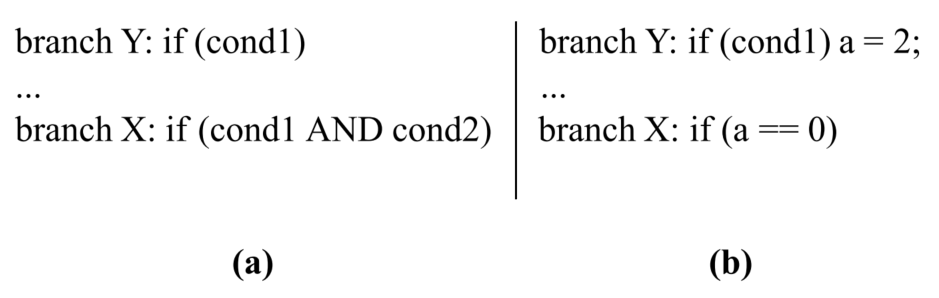
\includegraphics[width=0.5\linewidth]{assets/11/branch-direction-correlation.png}
  \caption{条件分支指令间的方向相关}
  \label{fig:branch-direction-correlation}
\end{figure}

除了方向相关外，不同的条件分支指令之间也存在路径相关。如图 \ref{fig:branch-path-correlation} 所示，假设
分支 X 不被分支 X、Z、V 控制（即无论分支 X、Z、V 跳转方向如何，分支 X 一定会
被执行），如果分支 V 被执行了，那么意味着分支 Y 和分支 Z 均未执行，因此无论分支
V 是否跳转，分支 X 一定执行跳转。分支 V 与分支 X 之间存在路径相关。

\begin{figure}[htbp]
  \centering
  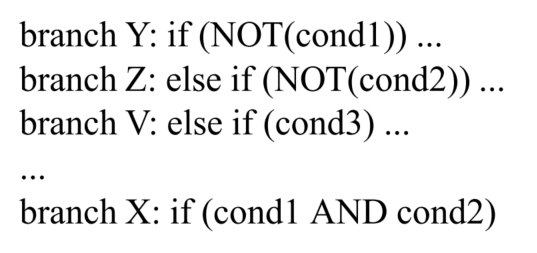
\includegraphics[width=0.5\linewidth]{assets/11/branch-path-correlation.png}
  \caption{条件分支指令间的路径相关}
  \label{fig:branch-path-correlation}
\end{figure}

针对条件分支指令存在的可预测性，历史上研究者们提出了很多种方法来预测条件分支指令的方向，本书将在 11.4.3 节中对此进行介绍。

由于无条件间接跳转类指令的跳转目标地址来自寄存器，直到执行时处理器才可以得知这类指令的跳转目标地址，因此有必要对此类指令的跳转目标地址进行预测。
一类容易预测的无条件间接跳转类指令是函数返回指令。由于函数调用与函数返回指令成对出现，且由于 ABI 的规定，函数调用与返回指令很容易被识别，因此可以用
一种特殊的存储结构存储函数的返回地址，这种结构一般被称为返回地址栈（Return Address Stack，RAS），本书将在 11.4.4 节对此进行介绍。

\subsection{分支目标缓冲}\label{sec:11-advanced-cpu-019}

分支目标缓冲（BTB）是分支预测器的核心，分支预测器中的其它组件都要依赖
BTB 提供的信息做出预测。由于 BTB 缓存分支指令的跳转地址及类型等信息，因此其
组织结构与高速缓存类似，可以实现为全相联、直接映射或多路组相联。在查询 BTB
时使用 PC 值的一部分作为索引（index）来寻址 BTB，PC 值的高位作为标签（tag）与
从 BTB 读出的表项中的标签域进行匹配生成命中或缺失信号。

\subsection{方向预测器}\label{sec:11-advanced-cpu-020}

方向预测器负责对条件分支指令的跳转方向做出预测。条件分支类指令往往是程序
执行过程中被执行次数最多的分支指令类型，其动态指令数往往远高于无条件跳转类指
令，因此对条件分支指令跳转方向的预测准确率会基本决定总体的分支预测准确率，从
而影响处理器性能。研究者们针对条件分支指令的方向预测进行了大量的研究。本节
将首先介绍最简单的方向预测器 BiModal 预测器，随后以 GShare 预测器为例引入全局分支历史的概念，最后介绍全局分
支历史的推测更新方式。

\subsubsection{BiModal 预测器}\label{sec:11-advanced-cpu-021}

BiModal 预测器是一种经典的条件分支方向预测器，它对条件分支指令的跳转倾向
进行预测。如图 \ref{fig:BiModal} 所示，它的主体是一个由一系列两位饱和计数器组成的模式历史
表（Pattern History Table，PHT），使用 PC 的低位索引 PHT，读出表项的最高位作为预
测的跳转方向，最高位为 1 表示跳转，为 0 表示不跳转。在更新时使用条件分支指令的
PC 索引 PHT，并根据指令的正确跳转方向更新对应的两位饱和计数器，当预测正确时
对计数器非上溢加一（即如果计数器值为 3 则不再加），当预测错误时对计数器非下溢
减一（即如果计数器值为 0 则不再减）。

\begin{figure}[htbp]
  \centering
  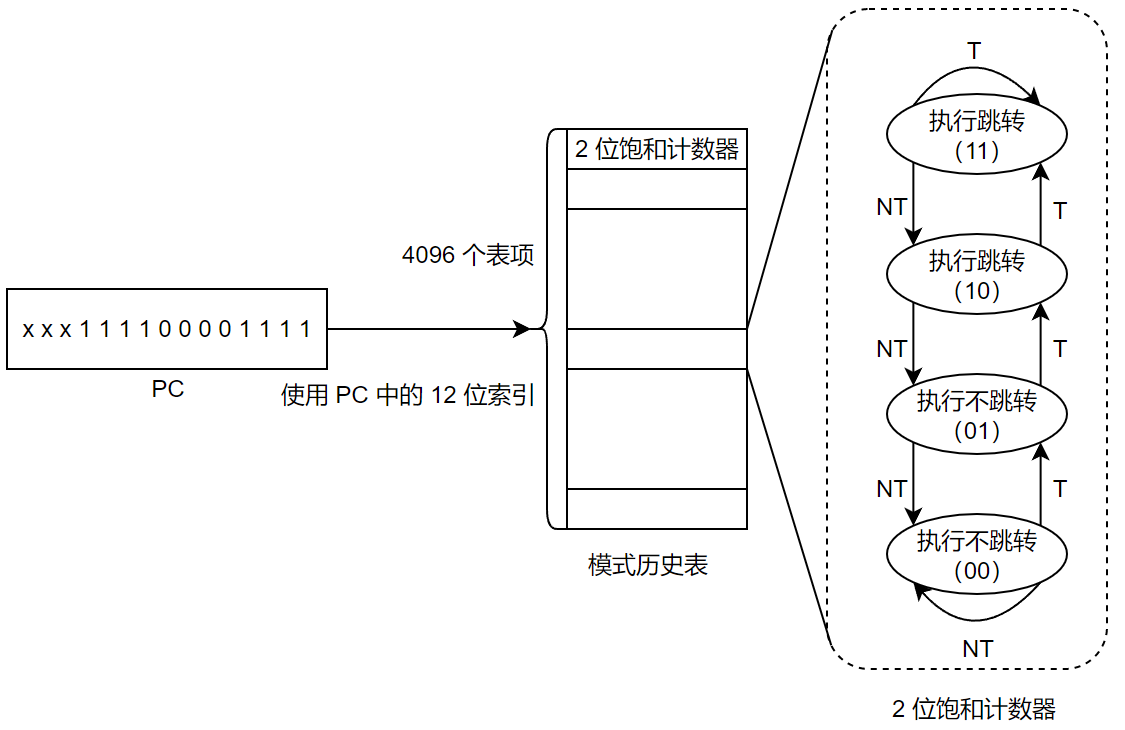
\includegraphics[width=0.5\linewidth]{assets/11/BiModal.png}
  \caption{BiModal 预测器}
  \label{fig:BiModal}
\end{figure}

BiModal 预测器仅考虑了分支指令自身跳转方向的倾向性，而忽略了分支指令自身
及不同分支指令跳转方向之间的许多潜在规律。因此其预测准确率不高，
BiModal 预测器在 SPEC CPU 1989 基准测试集上的平均预测准确率最高不到 94\%。

\subsubsection{使用全局模式历史------以 GShare 预测器为例}\label{sec:11-advanced-cpu-022}

可以使用一个全局的模式历史寄存器（Pattern History Register，PHR）来记录指令
流中条件分支指令的跳转方向。每执行一条条件分支指令，PHR 左移一位，并将最低位
置为该条条件分支的跳转方向（如跳转为 1，不跳转为 0）。如图 \ref{fig:GShare} 所示，GShare 预测
器将分支指令的 PC 中某些位（一般为 PC 的低位，也可以是 PC 哈希后的值）与 PHR
按位异或后得到的结果作为索引来选择 PHT 中的一个饱和计数器，然后将这个计数器
的最高位作为预测的跳转方向（如为 1 则跳转，否则不跳转）。更新时也通过同样的索
引方式索引到同一个饱和计数器进行更新。GShare 预测器的这种预测方式将不同全局
模式历史下的同一条分支指令的预测划分给了不同的饱和计数器，从而使得 GShare 预
测器可以捕捉单条分支指令自身跳转方向的规律性，以及不同条件分支指令之间的方向
相关性。

\begin{figure}[htbp]
  \centering
  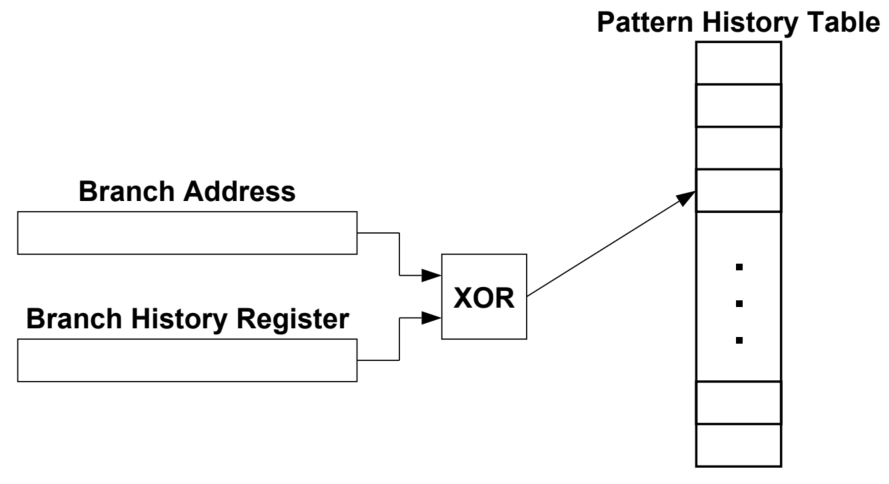
\includegraphics[width=0.5\linewidth]{assets/11/GShare.png}
  \caption{GShare 预测器}
  \label{fig:GShare}
\end{figure}

然而，GShare 预测器所需要的 PHT 表项个数与 PHR 的位宽呈指数关系，设 PHT
表项个数为 x，PHR 位宽为 y，则 \$ x = 2\^{}y \$。因此 PHR 每增加一位，PHT 表项数量需要增
加一倍。因此由于预测器面积与访问时间的限制，GShare 预测器无法使用较长的全局
模式历史，这限制了 GShare 预测器的准确率。

为了可以使用更长的全局模式历史，研究者们提出了很多预测器结构，如基于神经
网络的感知机预测器，基于 PPM 压缩算法的 PPM-like 预测器，使用呈几何级数长
度的全局分支历史的 O-GEHL 预测器，以及最终的集大成者 TAGE 预测器。目前
几乎所有的学术研究和商业高性能处理器都使用 TAGE 或者 TAGE 的变种作为提供高
准确率预测结果的条件分支预测器。

\subsubsection{推测更新全局模式历史}\label{sec:11-advanced-cpu-023}

在现代高性能处理器中的流水线中往往会同时存在上百条待执行的指令，而程序中
分支指令是较为密集的，通常平均每 5 到 10 条指令中就有一条是分支指令。因此如
果等待条件分支指令执行后，再根据执行结果更新全局模式历史寄存器，会导致在条件
分支指令被取进处理器流水线到被执行的这一段时间内，对在它后面被取进流水线的条
件分支指令进行跳转方向的预测时使用的不是最新的全局模式历史，从而极大的影响条
件分支预测器的预测准确率。

为了解决这一问题，目前普遍采用的做法是推测更新全局模式历史：当分支预测器
给出条件分支指令的方向预测结果后，立刻更新全局模式历史寄存器，从而保证每一次
预测都使用的是最新的全局模式历史。相应的，当检测到分支误预测时，需要对推测更
新的全局模式历史进行恢复。

\subsubsection{返回地址栈}\label{sec:11-advanced-cpu-024}

返回地址栈（Return Address Stack, RAS）是现代处理器中用于优化函数调用与返回性能的一种硬件结构。
它主要用于预测函数返回指令的目标地址，从而减少函数调用与返回过程中可能造成的流水线停顿。

在程序执行过程中，函数调用是一个非常常见的操作。当处理器执行函数调用指令时，
它会跳转到被调用函数的地址，并在函数执行完毕后返回调用点继续执行。
为了能够正确地返回调用点，处理器需要保存函数调用前的返回地址（即调用点的下一条指令的地址）。
然而，在深度流水线或多发射处理器中，等待函数返回指令的执行结果可能导致性能下降。
RAS 通过预测返回地址来缓解这一问题。RAS 的功能由函数调用时的地址存储、函数返回时的地址预测与
验证更新三部分组成：

\begin{itemize}
\tightlist
\item
  函数调用时的地址存储：当处理器遇到函数调用指令（如 BL/JIRL 指令）时，它会将返回地址（即函数调用后的指令地址）压入 RAS 中，同时跳转到被调用函数的地址。
\item
  函数返回时的地址预测：当处理器遇到函数返回指令（如 JIRL 指令）时，它会从 RAS 中弹出最顶端的地址，并预测这个地址是正确的返回地址。处理器然后使用这个预测地址来继续取指令并执行。
\item
  验证与更新：如果处理器预测的返回地址正确，执行继续而无需额外操作。如果预测错误，处理器需要回滚错误执行的指令，并将正确的返回地址更新到 RAS 中。
\end{itemize}
